\section{Results}
\label{sec:results}

\subsection{Inferred velocities}

To validate our method, we inferred velocities for stars in our sample with
measured RVs and compared those inferred values with velocities calculated
directly from 6D position, proper motion, and RV measurements.
Figure \ref{fig:residuals} shows the \vx, \vy\ and \vz\ velocities we
inferred, for 3000 stars chosen at random, compared with those calculated from
measured RVs.
\begin{figure}[ht!]
\caption{Vertical velocities calculated with full 6D information vs vertical
    velocities inferred without RVs, for 3000 \mct\ stars with \gaia\ RV
    measurements.}
  \centering
    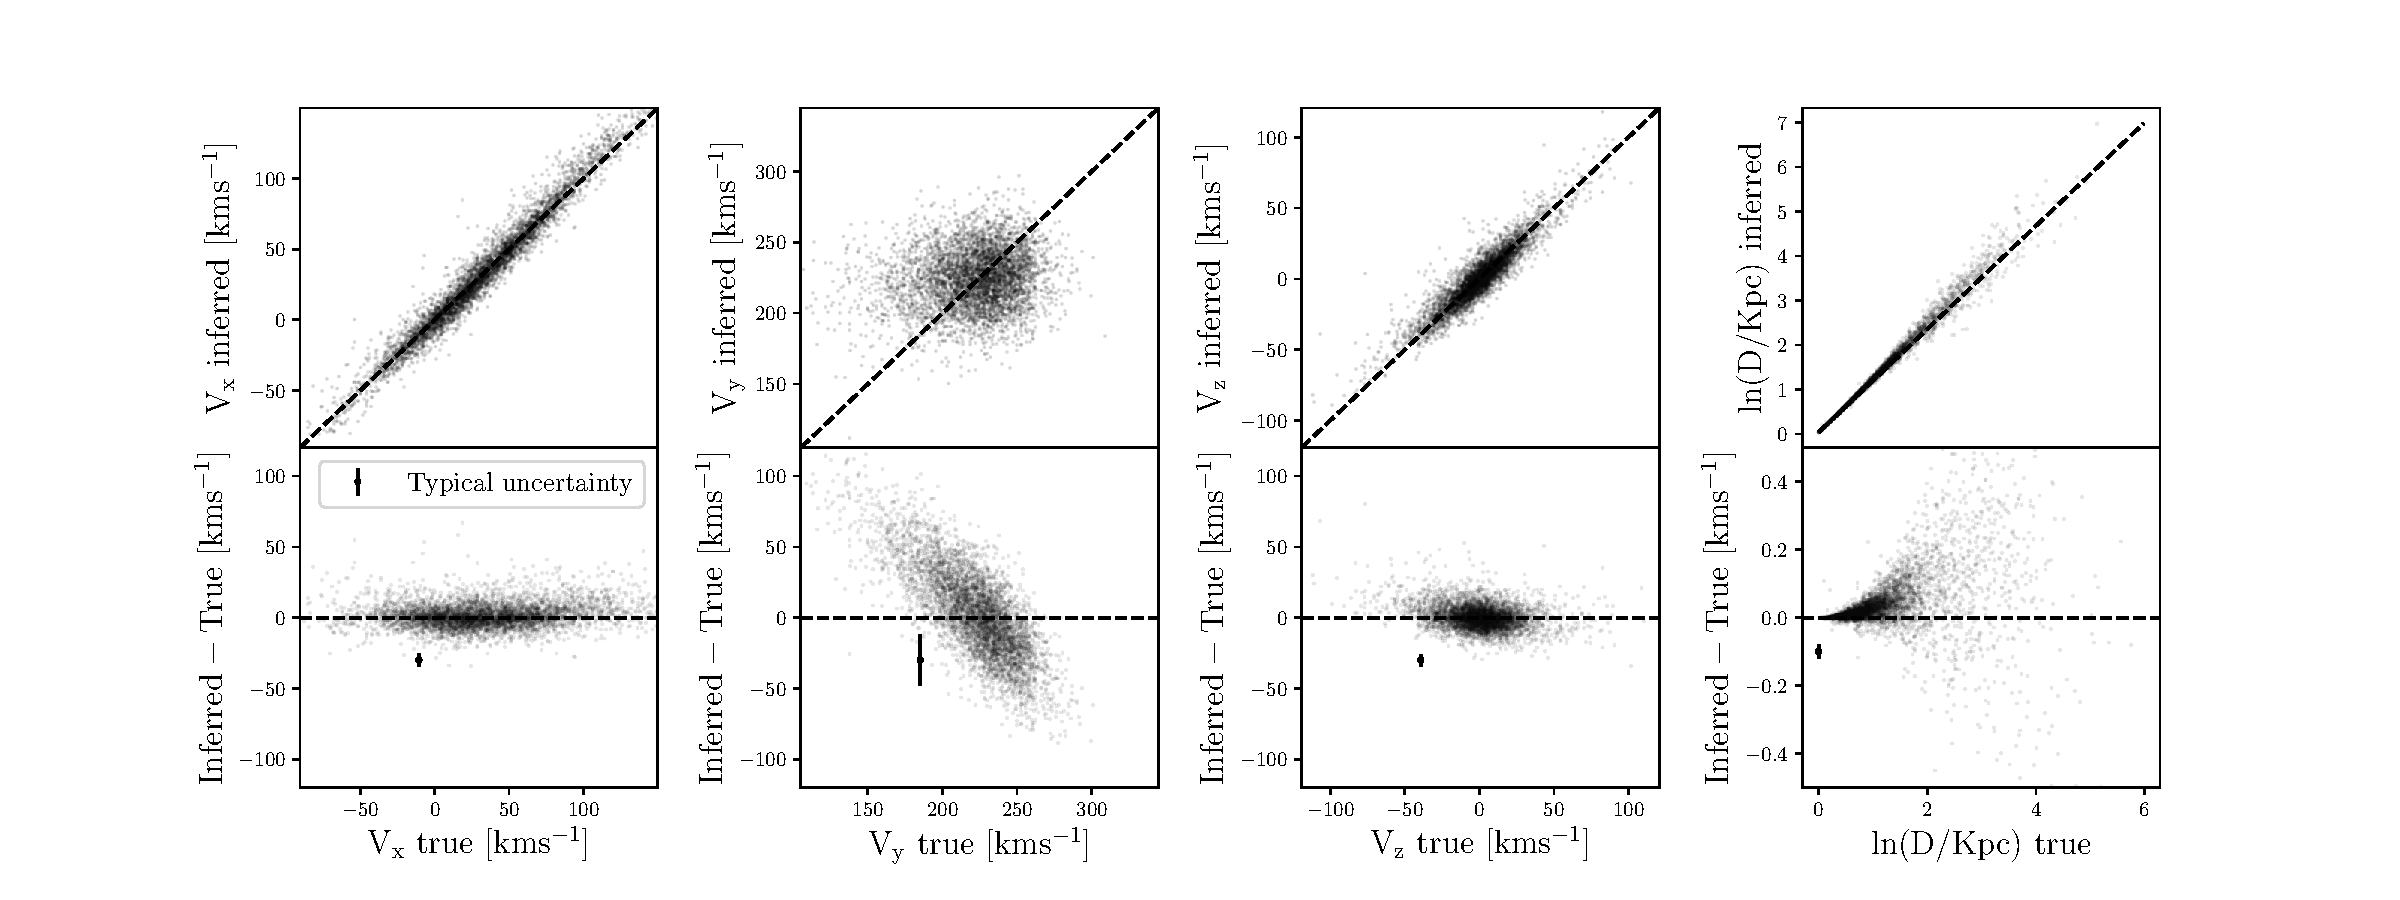
\includegraphics[width=1\textwidth]{residuals}
\label{fig:residuals}
\end{figure}

The three velocity components, \vx, \vy\ and \vz\ were recovered with
differing levels of precision: \vx\ and \vz\ are inferred more precisely than
\vy.
This is because of the orientation of the \kepler\ field, shown in figure
\ref{fig:kepler_field}.
\racomment{Slight inaccuracies seen in the residual panels for \vx\ and \vz\
are caused by ....
Quote some summary statistics.}

Table \ref{velocity_table} contains the inferred 3D velocities of stars in our
sample, in addition to their positional and velocity information from
Gaia EDR3, LAMOST DR5 and APOGEE DR16.
A sample of this table is displayed here, and the full machine-readable table
is available online.
